\documentclass[12pt]{article}
\usepackage{amsmath}
\usepackage{graphicx}
\usepackage{caption}
\usepackage{float}
\usepackage{geometry}
\geometry{margin=1in}

\title{CTA200 – Assignment 3 Writeup}
\author{Joely Ma}
\date{May 10th, 2025}

\begin{document}

\maketitle

\section*{Question 1: Iteration in the Complex Plane}

To explore the boundary between stability and divergence in a simple iterative system, I investigated the behavior of the recurrence relation:

\[
z_{i+1} = z_i^2 + c, \quad z_0 = 0
\]

for each complex number \( c = x + iy \) in the region \( -2 < x < 2 \), \( -2 < y < 2 \). For each \( c \), I applied this recurrence up to a fixed number of iterations (\( \text{max\_iter} = 100 \)) and recorded whether the absolute value of \( z \) exceeded 2. This allows us to visualize which starting values \( c \) cause the iteration to remain bounded and which cause it to diverge.

I implemented the iteration in a separate Python module and evaluated it across a uniform grid in the complex plane. In the first figure, I show a binary image where black points represent values of \( c \) that cause divergence within 100 iterations, and white points represent bounded trajectories.

To capture more detail, I then generated a second image where each point is colored according to the number of iterations it took for the sequence to diverge. This "escape-time" plot gives a smooth gradient and highlights the intricate boundary between stability and chaos.

These figures illustrate the sensitivity of this system to initial conditions and demonstrate fractal structure in a seemingly simple quadratic iteration.

\begin{figure}[H]
    \centering
    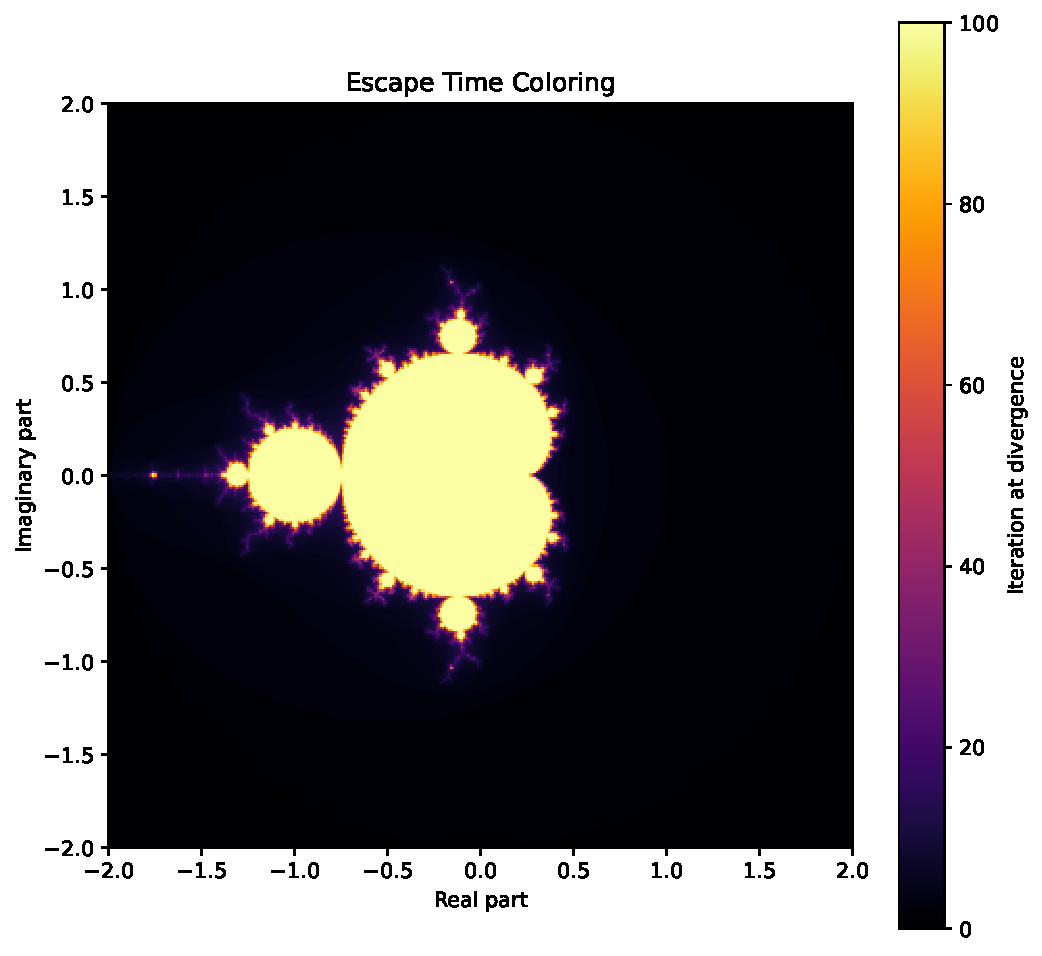
\includegraphics[width=\textwidth]{escape_time_plot.pdf}
    \caption{Escape-time coloring of complex iteration. Brighter colors indicate faster divergence.}
\end{figure}

\section*{Question 2: The Lorenz System}

The Lorenz system of differential equations models atmospheric convection in a simplified setting, capturing nonlinear dynamics and sensitivity to initial conditions. The equations are:

\[
\begin{aligned}
\dot{X} &= -\sigma(X - Y) \\
\dot{Y} &= rX - Y - XZ \\
\dot{Z} &= -bZ + XY
\end{aligned}
\]

I solved these equations using the Runge-Kutta method via \texttt{solve\_ivp} in Python’s \texttt{scipy} library. I used the standard Lorenz parameters (\( \sigma = 10 \), \( r = 28 \), \( b = \frac{8}{3} \)) and initial conditions \([0, 1, 0]\). The system was integrated over a time span of 60 time units with a step size of approximately 0.01.

Figure 1 in Lorenz’s original paper shows \( Y(t) \) over time. Our numerical reproduction reveals how the system begins with smooth oscillations and transitions into chaotic behavior. Small changes in the trajectory compound quickly, leading to an unpredictable long-term outcome even though the equations are deterministic.

\begin{figure}[H]
    \centering
    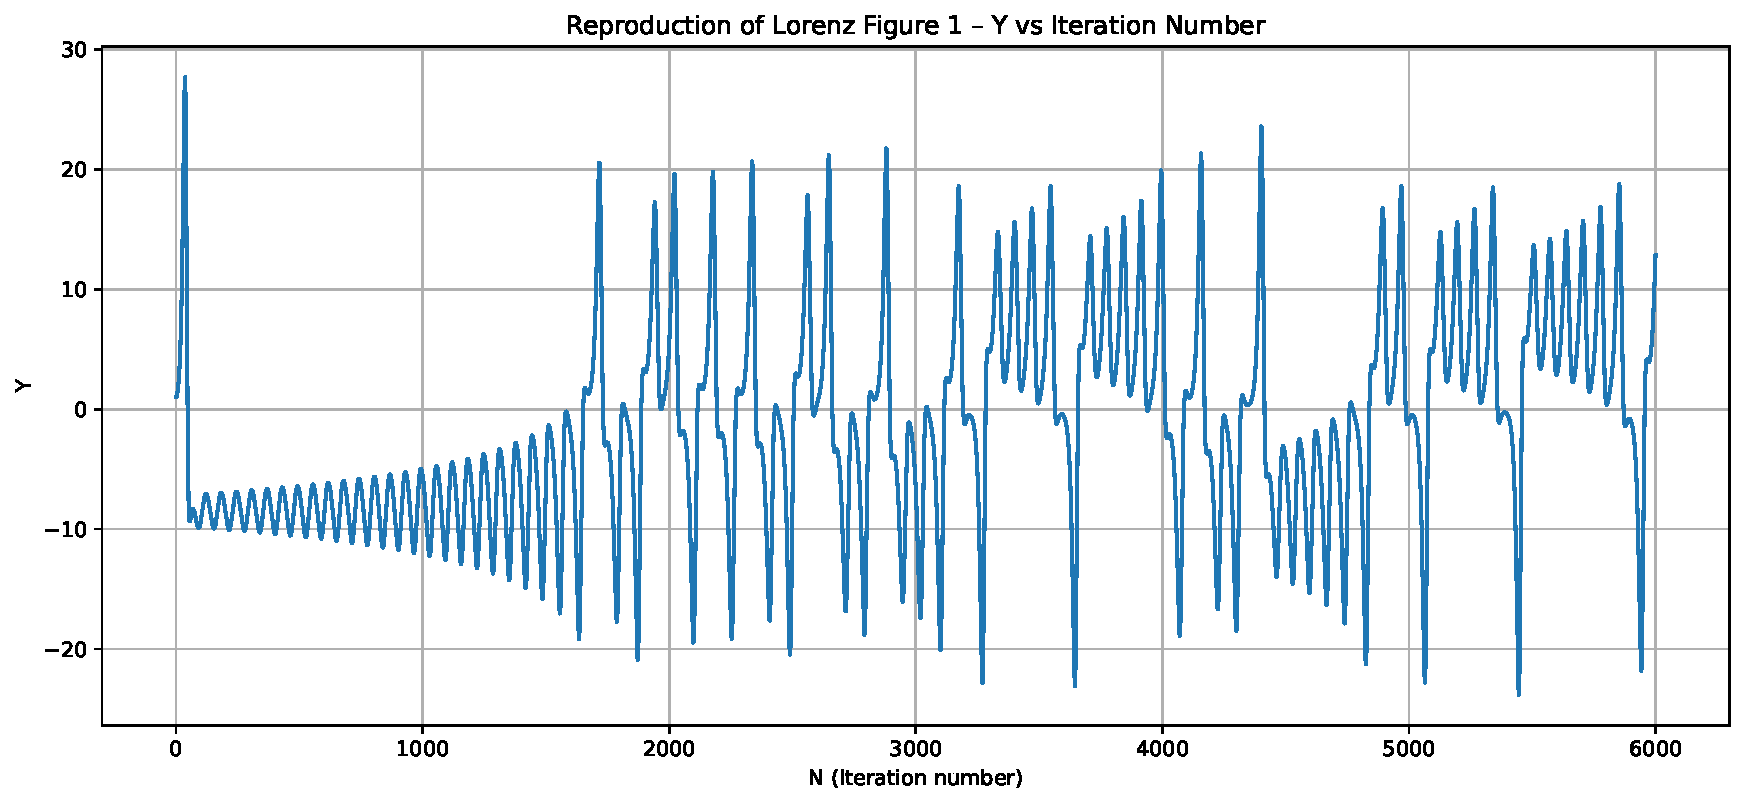
\includegraphics[width=\textwidth]{lorenz_y_vs_iter.pdf}
    \caption{Reproduction of Lorenz Figure 1: Y vs. iteration number \( N = t / 0.01 \).}
    \label{fig:lorenz1}
\end{figure}

To recreate Lorenz’s Figure 2, I extracted the segment of the trajectory corresponding to iteration numbers 1400 to 1900 (i.e., time \( t = 14 \) to \( t = 19 \)). I plotted two projections of the attractor: \( X \) vs. \( Y \) and \( Y \) vs. \( Z \). These phase-space diagrams show the "butterfly"-shaped structure for which the Lorenz system is famous, demonstrating how the state moves between two lobes in a chaotic, non-repeating pattern.

\begin{figure}[H]
    \centering
    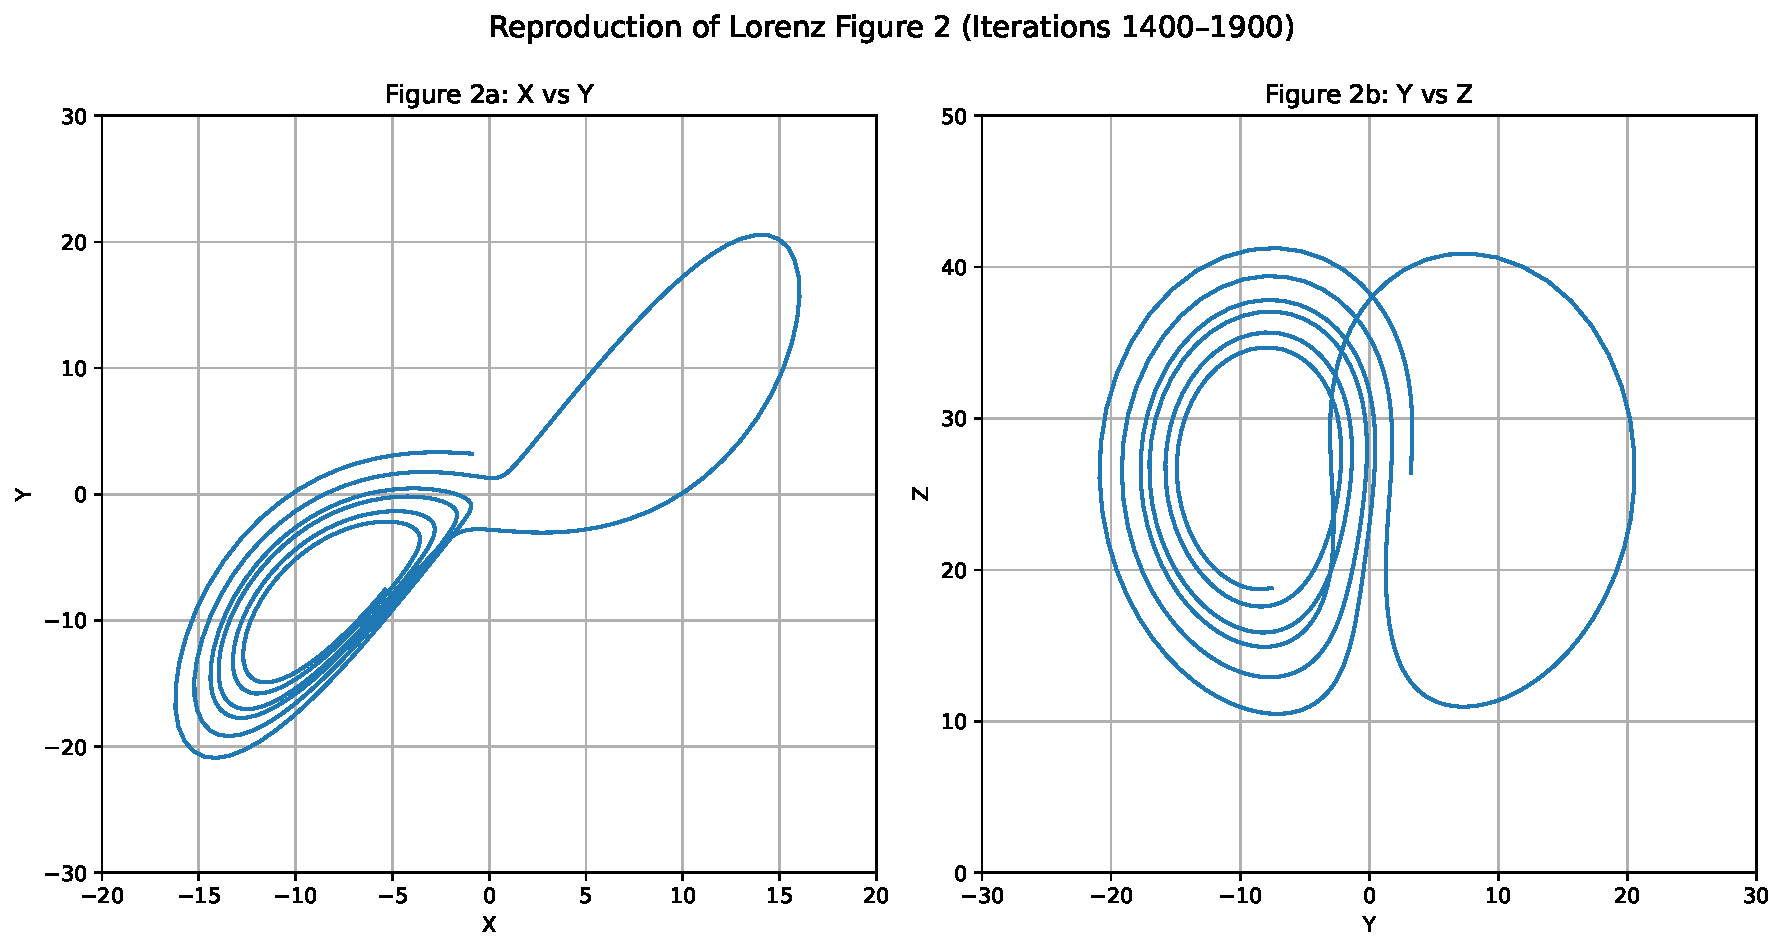
\includegraphics[width=\textwidth]{lorenz_y_vs_z.pdf}
    \caption{Reproduction of Lorenz Figure 2: X vs Y (left) and Y vs Z (right), for iterations 1400–1900.}
\end{figure}

\section*{Sensitivity to Initial Conditions}

To examine the chaotic nature of the Lorenz system, I repeated the simulation using an initial condition that was nearly identical to the original: \( [0.0, 1.00000001, 0.0] \). Despite the minuscule difference in \( Y_0 \), the trajectories of the two solutions diverged rapidly over time.

I computed the Euclidean distance between the two trajectories at each time point. Figure~\ref{fig:divergence} shows the results, with the Euclidean distance between the two trajectories plotted on a semilog scale using a logarithmic y-axis. This highlights the exponential rate of divergence typical of chaotic systems.. The linear trend in this plot confirms exponential divergence, which is a hallmark of chaos. This finding supports Lorenz’s conclusion that deterministic systems can exhibit unpredictable behavior due to extreme sensitivity to initial conditions — the so-called "butterfly effect."

\begin{figure}[H]
    \centering
    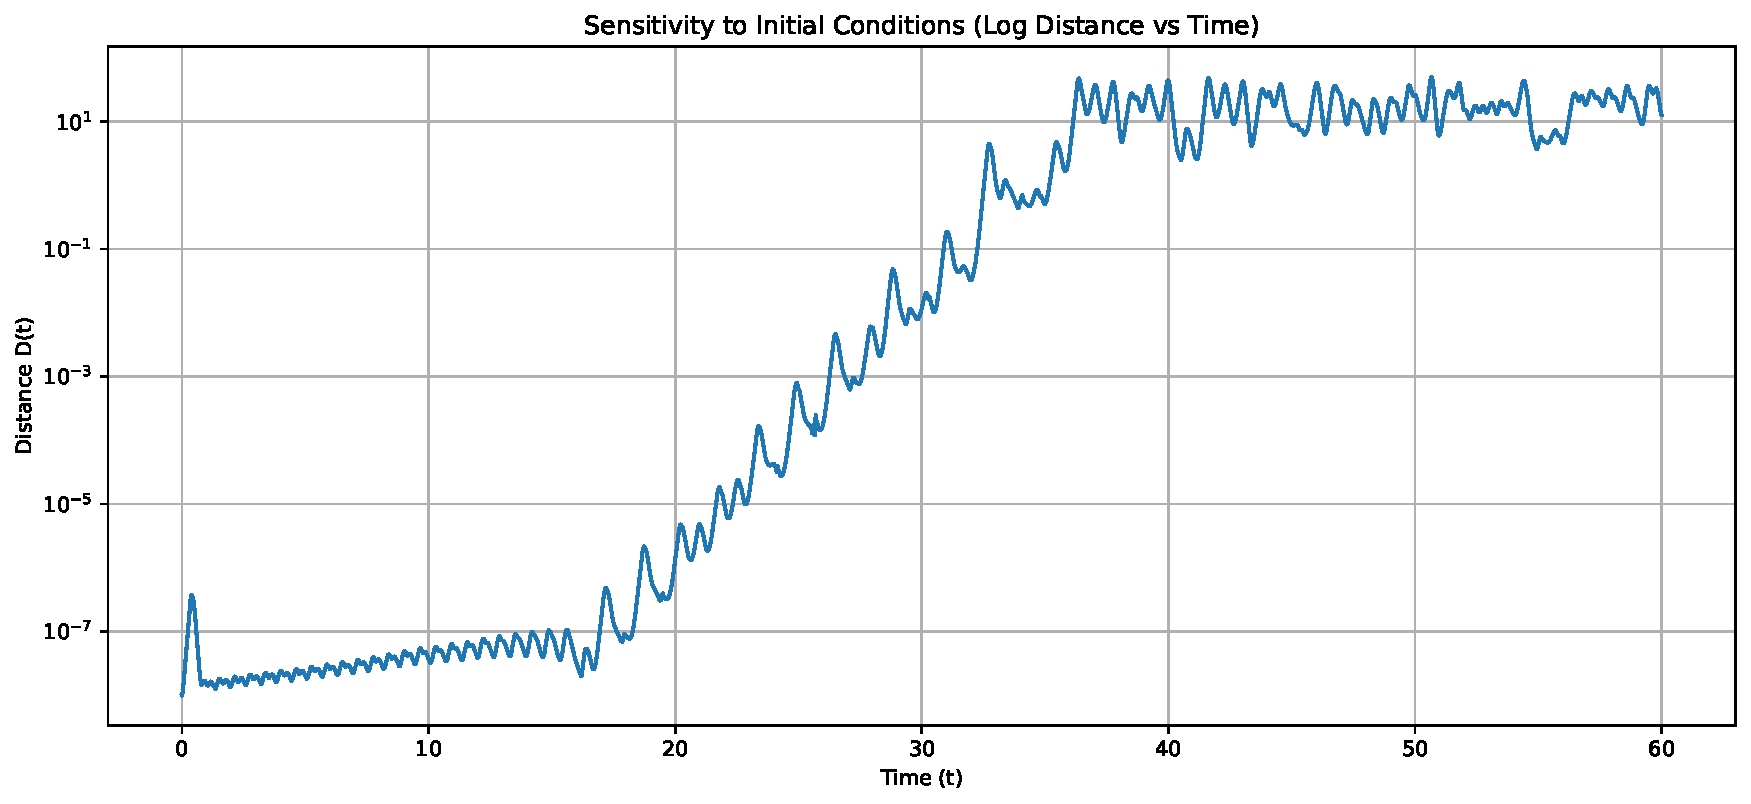
\includegraphics[width=\textwidth]{lorenz_log_distance.pdf}
    \caption{Log plot of distance between two Lorenz trajectories with slightly different initial conditions.}
    \label{fig:divergence}
\end{figure}

\end{document}